\documentclass[11pt,a4paper]{article}
\usepackage[utf8]{inputenc}
\usepackage[T1]{fontenc}
\usepackage{amsmath,amsfonts,amssymb}
\usepackage{graphicx}
\usepackage{xcolor}
\usepackage{booktabs}
\usepackage{array}
\usepackage{hyperref}
\usepackage{tikz}
\usetikzlibrary{arrows.meta,positioning,fit,backgrounds,calc}
\usepackage{fancybox}
\usepackage{enumitem}

\definecolor{darkblue}{RGB}{0,51,102}
\definecolor{priceblue}{RGB}{0,102,204}
\newcommand{\blue}[1]{\textcolor{priceblue}{\textbf{#1}}}
\newcommand{\gc}{\textbullet}

\begin{document}
	
	\section*{\centering Modular VHF-to-C-band Spectrum-Sensing Node}
	\noindent
	\section*{SDR and Processing Backend Selection}
	
	The proposed platform is a modular dual-receive-channel scanning node for
	VHF-to-C-band spectrum sensing. The architecture follows the design philosophy
	of SOSA (Sensor Open Systems Architecture) and related open-system approaches:
	standard RF interfaces, replaceable front-end modules, software-defined signal
	processing, and clear separation between the RF front-end, timing subsystem, and
	digital back-end.
	
	\medskip
	\noindent
	\textit{USRP N210 Networked SDR.}
	\begin{itemize}
		\item Dual-channel high-performance SDR with modular daughterboard architecture.
		The N210 motherboard provides a Xilinx Spartan-3A DSP 3400 FPGA with onboard
		digital downconversion (DDC) capability, Gigabit Ethernet host interface
		(\textbf{25~MS/s per channel} at 16-bit complex, \textbf{50~MS/s total}), and
		precision timing capabilities. Frequency coverage and instantaneous bandwidth are
		determined by the selected daughterboard(s).
		\item \textbf{Key advantage over USB-based SDRs:} Gigabit Ethernet provides
		reliable streaming over long cable runs (up to 100~m with standard cabling),
		reducing noise coupling and ground-loop issues compared to USB 3.0.
		\item Estimated price (used/refurbished): \blue{1,200--1,800 USD}.
		\href{https://www.ebay.com/itm/306170204276}{\gc}
		\item Daughterboard options for VHF-to-C-band coverage:
		\begin{itemize}
			\item \textbf{UBX (10~MHz--6~GHz):} Single daughterboard covering full
			VHF-to-C-band range. \textbf{2 TX / 2 RX ports} (both RX usable simultaneously
			for dual-branch). 40~MHz or 160~MHz instantaneous bandwidth. \\
			Estimated: \blue{800--1,200 USD} (used). \textbf{Recommended for simplicity.}
			\item \textbf{WBX + CBX pair:} Two daughterboards providing hardware-separated
			band optimization. WBX (50~MHz--2.2~GHz) for VHF/UHF branch, CBX (1.2--6~GHz)
			for UHF--C-band branch. Each provides 1 TX / 1 RX. \\
			Estimated: \blue{800--1,200 USD} combined (used). \textbf{Recommended for
				band isolation and reduced switching complexity.}
			\item \textbf{WBX (50~MHz--2.2~GHz):} Standalone for VHF/UHF coverage only.
			40~MHz or 120~MHz bandwidth. Estimated: \blue{400--600 USD} (used).
			\item \textbf{CBX (1.2~GHz--6~GHz):} Standalone for S/C-band coverage only.
			40~MHz or 120~MHz bandwidth. Estimated: \blue{400--600 USD} (used).
		\end{itemize}
		\item \textbf{Open-source advantage:} UHD (USRP Hardware Driver) is fully
		open-source under GPLv3, hosted on GitHub, with cross-platform support for
		GNU Radio, MATLAB, Python, and C/C++ development. SoapySDR provides a
		vendor-neutral abstraction layer compatible with UHD, bladeRF, RTL-SDR, and
		other devices.
	\end{itemize}
	
	\noindent
	\textit{Jetson Nano 4GB Developer Kit.}
	\begin{itemize}
		\item Compact embedded processing backend for FFT-based sensing, local control,
		metadata handling, and storage coordination. The 4GB LPDDR4 variant provides
		sufficient memory for multi-band spectral processing while maintaining low
		power consumption.
		\item Key specifications: Quad-core ARM Cortex-A57 @ 1.43~GHz, 128-core
		NVIDIA Maxwell GPU (472 GFLOPS), 4GB LPDDR4 @ 25.6 GB/s, Gigabit Ethernet,
		4x USB 3.0, 40-pin GPIO header (3.3V logic).
		\item Power envelope: 5W (default) to 10W (MAXN mode) via software-selectable
		power profiles. Requires 5V/4A barrel jack for MAXN mode; USB power
		insufficient for continuous operation.
		\item Estimated price: \blue{240--370 USD} (new, depending on vendor and
		availability).
	\end{itemize}
	
	\subsection*{Antenna System Configuration and RF Band Planning}
	
	Because the USRP N210 provides two receive channels via its daughterboard(s),
	the two main antenna paths can be assigned directly to separate RF inputs:
	\[
	\text{RX1} \leftarrow \text{VHF/UHF antenna path},
	\qquad
	\text{RX2} \leftarrow \text{UHF--C-band antenna path}.
	\]
	
	\textbf{With UBX daughterboard:} Both RX ports share identical 10~MHz--6~GHz
	coverage, enabling flexible band assignment entirely in software. This requires
	per-branch external preselection filters to isolate the target bands.
	
	\textbf{With WBX + CBX daughterboards:} RX1 (WBX) is hardware-limited to
	50~MHz--2.2~GHz; RX2 (CBX) to 1.2--6~GHz. This provides natural band
	separation, reducing filter bank complexity at the cost of dual-daughterboard
	synchronization.
	
	\begin{center}
		\fcolorbox{red!33}{gray!15}{%
			\begin{tabular}{c}
				\small
				VHF/UHF antenna
				\(\rightarrow\)
				Limiter/ESD
				\(\rightarrow\)
				VHF/UHF preselector
				\(\rightarrow\)
				LNA/bypass
				\(\rightarrow\)
				fixed attenuator pad
				\(\rightarrow\)
				USRP N210 RX1 (WBX or UBX)
			\end{tabular}
		}
	\end{center}
	
	\begin{center}
		\fcolorbox{red!33}{gray!15}{%
			\begin{tabular}{c}
				\small
				UHF--C-band antenna
				\(\rightarrow\)
				Limiter/ESD
				\(\rightarrow\)
				UHF/S-band/C-band preselector bank
				\(\rightarrow\)
				LNA/bypass
				\(\rightarrow\)
				fixed attenuator pad
				\(\rightarrow\)
				USRP N210 RX2 (CBX, SBX, or UBX)
			\end{tabular}
		}
	\end{center}
	
	\begin{table}[htbp]
		\centering
		\small
		\begin{tabular}{@{}lllll@{}}
			\toprule
			\textbf{Band} &
			\textbf{Antenna Type} &
			\textbf{Model Example} &
			\textbf{Frequency Range} &
			\textbf{Gain} \\
			\midrule
			
			VHF/UHF survey &
			Biconical &
			Aaronia BicoLOG 5070
			\blue{100 USD}
			\href{https://aaroniausa.com/product/antennas/biconical-antennas/bicolog-5070-radial-isotropic/}{\gc} &
			70 MHz--700 MHz &
			$\sim$0 dBi \\
			
			UHF--C-band survey &
			Log-periodic &
			Aaronia HyperLOG 7060
			\blue{320--540 USD}
			\href{https://thedebugstore.com/products/aaronia-hyperlog-7000-series-700mhz-6ghz-log-periodic-antenna}{\gc} &
			700 MHz--6 GHz &
			5--7 dBi \\
			
			\bottomrule
		\end{tabular}
		\caption{Antenna selection for the modular dual-branch spectrum-sensing node.}
		\label{tab:antenna-selection}
	\end{table}
	
	\subsection*{Supporting Hardware}
	
	\[
	\textit{Laboratory prototype:}\quad
	\text{simplified preselection, optional FM notch, LNA/bypass, fixed SMA attenuator pads.}
	\]
	\[
	\textit{Field-usable node:}
	\quad
	\text{per-branch modular filter bank, calibrated paths, automated RF switching, programmable attenuators.}
	\]
	
	\begin{enumerate}[label=\roman*)]
		
		\item \textbf{Low-noise amplifiers and bypass strategy.}
		
		The LNA subsystem is divided into frequency-dependent gain paths. Each LNA path
		should include a bypass state so that the receiver can avoid front-end
		compression when strong in-band or out-of-band signals are present. This is
		especially important near FM broadcast transmitters, cellular base stations,
		telemetry sources, or other high-power emitters.
		
		For the USRP N210-based dual-branch architecture, the LNA/bypass strategy should
		be implemented independently in each receive branch. The VHF/UHF branch can use
		a wideband low-noise amplifier covering the lower bands, while the UHF--C-band
		branch requires separate gain paths for the lower microwave, \textbf{3--4 GHz
			(specified with concrete catalog part)}, and upper C-band regions. In all
		cases, the LNA should be placed after the limiter/ESD protection and after the
		selected preselector filter, so that strong out-of-band signals are attenuated
		before gain is applied.
		
		\begin{table}[!ht]
			\centering
			\small
			\begin{tabular}{p{4.1cm}p{2.4cm}p{1.7cm}p{1.5cm}p{4.7cm}}
				\toprule
				\textbf{Model} &
				\textbf{Range} &
				\textbf{Gain} &
				\textbf{NF} &
				\textbf{Use Case} \\
				\midrule
				
				Mini-Circuits ZX60-33LN-S+
				\blue{159 USD}
				\href{https://www.minicircuits.com/WebStore/dashboard.html?model=ZX60-33LN-S\%2B}{\gc} &
				50 MHz--3 GHz &
				20 dB &
				3 dB &
				VHF, UHF, and lower microwave sensing. \\
				
				\textbf{Mini-Circuits SBP-3800+}
				\blue{45--65 USD} &
				3.0--4.2 GHz &
				-- &
				-- &
				\textbf{3--4 GHz bandpass filter. Closes coverage gap with
					concrete catalog part. 50-ohm SMA, hermetic LTCC construction.} \\
				
				Additional 3--4 GHz LNA
				\blue{50--150 USD} &
				3 GHz--4 GHz &
				15--25 dB &
				TBD &
				Closes the coverage gap between the lower wideband LNA and the upper
				microwave/C-band LNA path. \\
				
				Amplitech AGLNA035082
				\blue{35 USD}
				\href{https://shop.amplitechinc.com/collections/lna-s}{\gc} &
				4.0 GHz--8.0 GHz &
				26 dB typ. &
				0.9 dB &
				Upper microwave and C-band sensing. \\
				
				\bottomrule
			\end{tabular}
			\caption{Frequency-dependent LNA paths. Each gain path should include a bypass state.
				\textbf{Note:} SBP-3800+ specified as concrete catalog part for 3--4 GHz preselection.}
			\label{tab:lna-selection}
		\end{table}
		
		For cost-effective implementation, the first prototype may use a manual or
		semi-automatic LNA/bypass selection network. A fully automated version should
		use solid-state RF switches (see below) so that the software controller can
		select high-sensitivity, protected, or calibration modes according to the
		measured input-power conditions.
		
		\item \textbf{Preselection and band plan.}
		
		Although the USRP N210 with UBX daughterboard provides wide tuning coverage from
		approximately 10~MHz to 6~GHz, this tuning range does not by itself provide
		sufficient external RF selectivity. In realistic RF environments, strong
		out-of-band signals may drive the LNA or SDR input toward compression before
		digitization. Therefore, external preselection remains necessary when the node
		is intended for field deployment, repeatable measurements, or operation near
		high-power emitters.
		
		For the USRP N210-based dual-branch architecture, the filter bank should be
		interpreted as a per-branch preselection network rather than as a single
		centralized RF path. The VHF/UHF branch should include low-VHF/VHF/UHF
		preselection and a switchable FM notch or FM pass path. The UHF--C-band branch
		should use replaceable filter modules for upper-UHF, cellular/ISM, S-band, and
		C-band sensing. This preserves modularity while avoiding unnecessary centralized
		antenna switching.
		
		\begin{table}[htbp]
			\centering
			\small
			\begin{tabular}{p{2.4cm}p{3.1cm}p{2.5cm}p{1.6cm}p{4.9cm}}
				\toprule
				\textbf{Sensing Region} &
				\textbf{Suggested Filter Path} &
				\textbf{Nominal Band} &
				\textbf{Typ. IL} &
				\textbf{Purpose and Comments} \\
				\midrule
				
				70--88 MHz &
				Low-VHF preselector or broad VHF path &
				70--88 MHz &
				TBD &
				Lower-VHF sensing below the FM broadcast band. \\
				
				88--108 MHz &
				Switchable FM notch or FM pass path &
				88--108 MHz &
				$<$1.5 dB pass &
				The FM notch protects the receiver during wideband surveys, but must be
				bypassed when FM broadcast monitoring is the target. \\
				
				108--700 MHz &
				Mini-Circuits SHP-50+ + SLP-750+
				\href{https://www.minicircuits.com}{\gc} &
				108--700 MHz &
				$\sim$2 dB &
				General VHF/UHF monitoring with reduced low-frequency and out-of-band
				loading before amplification. \\
				
				700--960 MHz &
				Modular BPF or cavity filter &
				700--960 MHz &
				$<$2 dB &
				Mobile, public-safety, telemetry, and upper-UHF services. A replaceable
				SMA filter module is preferred over a fixed custom-only part. \\
				
				1.7--2.7 GHz &
				Custom BPF or partial VBFZ-2130-S+ path
				\href{https://www.minicircuits.com}{\gc} &
				1.7--2.7 GHz &
				$<$2 dB &
				Common cellular, ISM, and microwave communication regions. The final
				filter should match the exact services to be monitored. \\
				
				\textbf{3.0--4.2 GHz} &
				\textbf{Mini-Circuits SBP-3800+}
				\blue{45--65 USD} &
				\textbf{3.0--4.2 GHz} &
				\textbf{$<$3 dB} &
				\textbf{Closes the 3--4 GHz coverage gap with specified catalog part.
					LTCC bandpass filter, 50-ohm SMA, hermetic.} \\
				
				4.0--6.0 GHz &
				Marki Microwave C-band BPF or equivalent
				\href{https://shop.markimicrowave.com}{\gc} &
				4--6 GHz &
				$<$3 dB &
				Focused C-band sensing. This module should remain replaceable because
				C-band monitoring requirements may vary by application and region. \\
				
				\bottomrule
			\end{tabular}
			\caption{Modular RF band plan for VHF-to-C-band spectrum sensing.
				\textbf{Note:} SBP-3800+ specified as concrete catalog part for 3--4 GHz gap.}
			\label{tab:rf-band-plan}
		\end{table}
		
		The RF front-end should support at least three operating modes. In the
		USRP N210-based architecture, these modes may be applied independently to each
		receive branch, depending on the target band and the measured input-power
		conditions:
		\begin{enumerate}
			\item \textbf{Wideband survey mode:} moderate gain, conservative attenuation,
			and broad preselection for spectrum-occupancy mapping across the assigned
			receive branch.
			
			\item \textbf{Protected urban mode:} FM-notch or band-limiting preselection
			enabled when appropriate, LNA bypass available, and increased attenuation to
			avoid front-end or SDR-input compression.
			
			\item \textbf{Focused band-analysis mode:} narrow preselector enabled, LNA path
			selected according to the target band, and attenuation adjusted so that the
			LNA and SDR input remain within their linear operating ranges.
		\end{enumerate}
		
		\item \textbf{RF-path switching -- solid-state SP4T for deployable nodes.}
		
		For a deployable node, per-branch RF switching is implemented using
		\textbf{solid-state SP4T switches}. The following catalog parts are specified:
		
		\begin{itemize}
			\item \textbf{Mini-Circuits MSW-2-50DR+} or equivalent Qorvo/RFMD solid-state
			SP4T switch. DC--5~GHz coverage, low insertion loss ($<$2~dB), high isolation
			($>$30~dB), \textbf{3.3V CMOS logic control} (directly compatible with Jetson
			Nano GPIO without level shifters). Estimated: \blue{25--40 USD} (qty 1).
			\item \textbf{Alternative:} Mini-Circuits ZSWA-4-50DR+ (SP4T, DC--5~GHz) or
			Skyworks SKY13453-385LF (SP4T, 0.1--6~GHz, $>$35~dB isolation, 1.8--3.3V control).
			\item Control interface: Direct 3.3V CMOS from Jetson Nano GPIO pins, or SPI
			via USB-SPI bridge for expanded channel count.
		\end{itemize}
		
		\textbf{Prototype phase:} For the laboratory prototype, manual SMA patch-cord
		routing between filter modules is acceptable. This eliminates switch cost and
		complexity while preserving modularity. \textbf{Power impact:} 0~W (passive
		routing) vs. 0.2--0.6~W (solid-state switches).
		
		\item \textbf{Attenuation strategy -- fixed pads for prototype, programmable for deployment.}
		
		\textbf{Prototype phase (fixed SMA attenuator pads):}
		\begin{itemize}
			\item Mini-Circuits \textbf{UNAT-1+} (1~dB), \textbf{UNAT-3+} (3~dB),
			\textbf{UNAT-6+} (6~dB), \textbf{UNAT-10+} (10~dB). DC--6~GHz, 2~W power
			handling, SMA male-to-female connectors.
			\item Estimated cost per pad: \blue{8--15 USD}. A kit of 4 values per branch
			(8 pads total): \blue{64--120 USD} total.
			\item Implementation: Manual selection and insertion between LNA output and
			USRP RX input. Suitable for laboratory prototype where automatic gain control
			is not required.
		\end{itemize}
		
		\textbf{Deployable phase (programmable step attenuators):}
		\begin{itemize}
			\item Mini-Circuits \textbf{ZX76-31R75PP-S+} (DC--6~GHz, 0--31.5~dB, 0.5~dB
			steps) or equivalent. Estimated: \blue{300--350 USD} each.
			\item Two units recommended (one per branch) for symmetric gain management.
			Total: \blue{600--700 USD}.
			\item \textbf{Deferred to Phase 2:} Programmable attenuators are not required
			for the initial prototype. Budget for them in the deployable revision.
		\end{itemize}
		
		\item \textbf{Timing and synchronization.}
		
		The USRP N210 provides flexible timing options:
		\begin{itemize}
			\item \textbf{Onboard TCXO:} $\sim$2.5~ppm frequency accuracy (sufficient
			for many sensing applications).
			\item \textbf{Optional internal GPSDO:} Ettus Research GPSDO module provides
			$<$50~ppb when locked. Estimated: \blue{400--600 USD} (used, if not included
			with N210).
			\item \textbf{External reference:} 10~MHz and 1~PPS inputs on rear panel.
			The N210 accepts \textbf{5~MHz or 10~MHz external references at 0.5--3.3Vpp
				(sine or CMOS)} directly via SMA---no adapter cables needed.
			\item \textbf{Leo Bodnar Precision GPSDO (external):} \blue{150 USD}
			\href{https://leobodnar.com/shop/index.php?main_page=product_info\&products_id=301}{\gc}.
			Outputs 10~MHz (3.3V CMOS) and 1~PPS. Connects directly to N210 rear-panel
			REF IN via SMA. \textbf{Voltage level compatible without additional conditioning.}
			\item The GPS lock state and reference-lock state should be logged as part of
			the sensing metadata.
		\end{itemize}
		
	\end{enumerate}
	
	\subsection*{System Block Diagram}
	
	The following diagram illustrates the complete USRP N210 + Jetson Nano
	architecture, highlighting Ethernet streaming (vs. USB 3.0 in bladeRF systems),
	direct SMA timing reference, and per-branch modular RF front-end.
	
	\begin{center}
		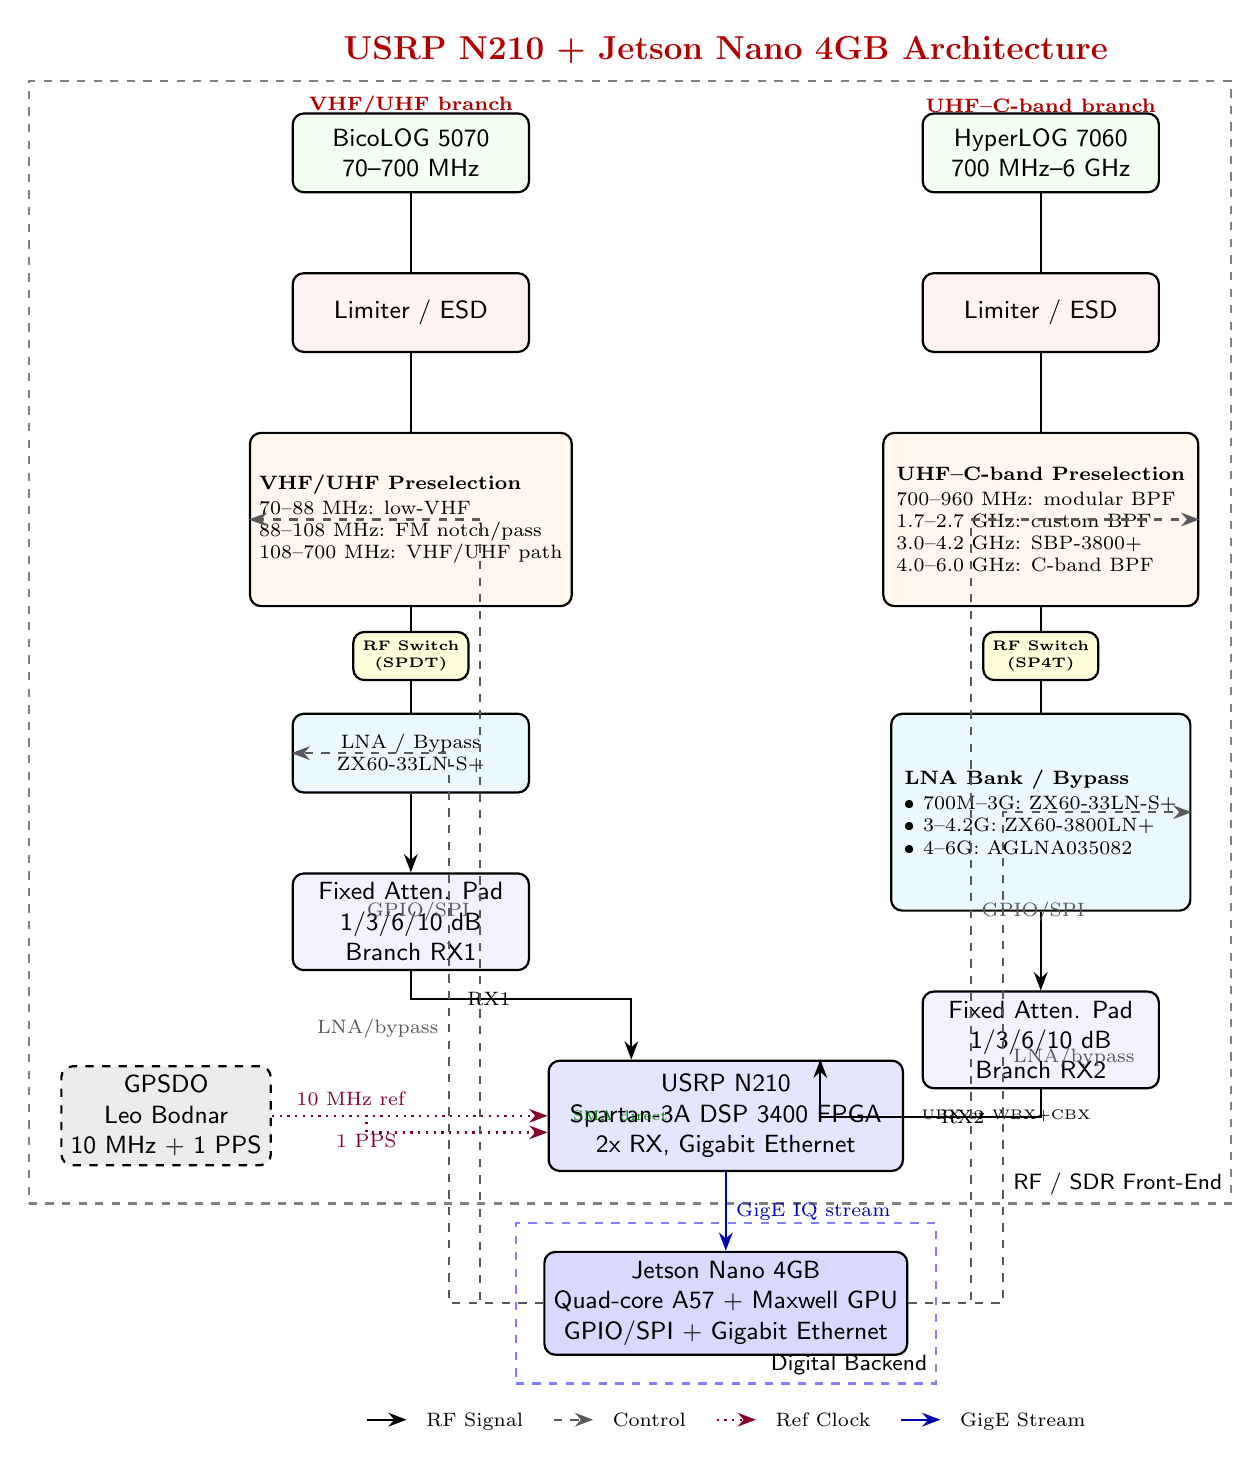
\begin{tikzpicture}[
			font=\small\sffamily,
			>=Stealth,
			antblock/.style={draw, thick, fill=green!5, rounded corners, minimum height=1.0cm, minimum width=3.0cm, align=center},
			protblock/.style={draw, thick, fill=red!5, rounded corners, minimum height=1.0cm, minimum width=3.0cm, align=center},
			filterblock/.style={draw, thick, fill=orange!7, rounded corners, minimum height=2.2cm, minimum width=4.0cm, align=left, font=\scriptsize},
			switchblock/.style={draw, thick, fill=yellow!15, rounded corners, minimum height=0.6cm, minimum width=1.4cm, align=center, font=\tiny\bfseries},
			lnablock/.style={draw, thick, fill=cyan!8, rounded corners, minimum height=1.0cm, minimum width=3.0cm, align=center, font=\scriptsize},
			lnabankblock/.style={draw, thick, fill=cyan!8, rounded corners, minimum height=2.5cm, minimum width=3.8cm, align=left, font=\scriptsize},
			attblock/.style={draw, thick, fill=blue!5, rounded corners, minimum height=1.0cm, minimum width=3.0cm, align=center},
			sdrblock/.style={draw, thick, fill=blue!10, rounded corners, minimum height=1.4cm, minimum width=4.5cm, align=center},
			procblock/.style={draw, thick, fill=blue!15, rounded corners, minimum height=1.0cm, minimum width=3.5cm, align=center},
			gpsdoblock/.style={draw, thick, fill=gray!15, dashed, rounded corners, minimum height=0.9cm, minimum width=2.5cm, align=center},
			annot/.style={font=\scriptsize\bfseries, text=red!70!black},
			arrow/.style={thick,->},
			ctrlarrow/.style={thick,dashed,->,gray!70!black},
			refarrow/.style={thick,dotted,->,purple!70!black},
			etharrow/.style={thick,->,blue!70!black},
			node distance=1.0cm and 1.4cm
			]
			
			% Title
			\node[font=\large\bfseries,text=red!70!black] at (5.5,10.5)
			{USRP N210 + Jetson Nano 4GB Architecture};
			
			% LEFT BRANCH (VHF/UHF)
			\node[annot] at (1.5,9.8) {VHF/UHF branch};
			\node[antblock] (ant1) at (1.5,9.2) {BicoLOG 5070\\70--700 MHz};
			\node[protblock,below=of ant1] (lim1) {Limiter / ESD};
			\node[filterblock,below=of lim1] (filt1) {
				\textbf{VHF/UHF Preselection}\\[1pt]
				70--88 MHz: low-VHF\\
				88--108 MHz: FM notch/pass\\
				108--700 MHz: VHF/UHF path
			};
			\node[switchblock,below=0.3cm of filt1] (sw1) {RF Switch\\(SPDT)};
			\node[lnablock,below=0.4cm of sw1] (lna1) {LNA / Bypass\\ZX60-33LN-S+};
			\node[attblock,below=of lna1] (att1) {Fixed Atten. Pad\\1/3/6/10 dB\\Branch RX1};
			
			% RIGHT BRANCH (UHF--C-band)
			\node[annot] at (9.5,9.8) {UHF--C-band branch};
			\node[antblock] (ant2) at (9.5,9.2) {HyperLOG 7060\\700 MHz--6 GHz};
			\node[protblock,below=of ant2] (lim2) {Limiter / ESD};
			\node[filterblock,below=of lim2] (filt2) {
				\textbf{UHF--C-band Preselection}\\[1pt]
				700--960 MHz: modular BPF\\
				1.7--2.7 GHz: custom BPF\\
				3.0--4.2 GHz: SBP-3800+\\
				4.0--6.0 GHz: C-band BPF
			};
			\node[switchblock,below=0.3cm of filt2] (sw2) {RF Switch\\(SP4T)};
			\node[lnabankblock,below=0.4cm of sw2] (lna2) {
				\textbf{LNA Bank / Bypass}\\[1pt]
				\textbullet\ 700M--3G: ZX60-33LN-S+\\
				\textbullet\ 3--4.2G: ZX60-3800LN+\\
				\textbullet\ 4--6G: AGLNA035082
			};
			\node[attblock,below=of lna2] (att2) {Fixed Atten. Pad\\1/3/6/10 dB\\Branch RX2};
			
			% USRP N210 (CENTER)
			\node[sdrblock,below=1.0cm of $(att1)!0.5!(att2)$] (sdr) {USRP N210\\
				Spartan-3A DSP 3400 FPGA\\
				2x RX, Gigabit Ethernet};
			
			% Daughterboard annotation
			\node[font=\tiny,right=0.1cm of sdr.east] {UBX or WBX+CBX};
			
			% Jetson Nano
			\node[procblock,below=of sdr] (jetson) {Jetson Nano 4GB\\
				Quad-core A57 + Maxwell GPU\\
				GPIO/SPI + Gigabit Ethernet};
			
			% GPSDO
			\node[gpsdoblock,left=3.5cm of sdr] (gpsdo) {GPSDO\\Leo Bodnar\\10 MHz + 1 PPS};
			
			% RF paths
			\draw[arrow] (ant1) -- (lim1) -- (filt1) -- (sw1) -- (lna1) -- (att1);
			\draw[arrow] (att1.south) -- ++(0,-0.35) -| node[pos=0.25,left,font=\scriptsize] {RX1} ([xshift=-1.2cm]sdr.north);
			\draw[arrow] (ant2) -- (lim2) -- (filt2) -- (sw2) -- (lna2) -- (att2);
			\draw[arrow] (att2.south) -- ++(0,-0.35) -| node[pos=0.25,right,font=\scriptsize] {RX2} ([xshift=1.2cm]sdr.north);
			
			% Ethernet streaming (KEY DIFFERENCE from bladeRF)
			\draw[etharrow] (sdr) -- node[right,font=\scriptsize] {GigE IQ stream} (jetson);
			
			% Reference timing
			\draw[refarrow] (gpsdo.east) -- ++(1.0,0) |- node[pos=0.25,above,font=\scriptsize] {10 MHz ref} (sdr.west);
			\draw[refarrow] (gpsdo.east) -- ++(1.2,0) |- node[pos=0.25,below,font=\scriptsize] {1 PPS} ([yshift=-6pt]sdr.west);
			\node[font=\tiny,text=green!50!black,right=0.2cm of sdr.west] {SMA direct};
			
			% Control paths
			\draw[ctrlarrow] (jetson.west) -- ++(-0.8,0) |- node[pos=0.25,left,font=\scriptsize] {GPIO/SPI} (filt1.west);
			\draw[ctrlarrow] (jetson.west) -- ++(-1.2,0) |- node[pos=0.25,left,font=\scriptsize] {LNA/bypass} (lna1.west);
			\draw[ctrlarrow] (jetson.east) -- ++(0.8,0) |- node[pos=0.25,right,font=\scriptsize] {GPIO/SPI} (filt2.east);
			\draw[ctrlarrow] (jetson.east) -- ++(1.2,0) |- node[pos=0.25,right,font=\scriptsize] {LNA/bypass} (lna2.east);
			
			% System boundaries
			\begin{scope}[on background layer]
				\node[draw, thick, dashed, gray, fit=(ant1)(ant2)(lim1)(lim2)(filt1)(filt2)(sw1)(sw2)(lna1)(lna2)(att1)(att2)(sdr)(gpsdo), inner sep=0.4cm, label={[anchor=south east]south east:{\footnotesize RF / SDR Front-End}}] {};
				\node[draw, thick, dashed, blue!50, fit=(jetson), inner sep=0.35cm, label={[anchor=south east]south east:{\footnotesize Digital Backend}}] {};
			\end{scope}
			
			% Legend
			\node[below=0.6cm of jetson, font=\scriptsize] {
				\tikz\draw[thick,->] (0,0) -- (0.5,0); \, RF Signal \quad
				\tikz\draw[thick,dashed,->,gray!70!black] (0,0) -- (0.5,0); \, Control \quad
				\tikz\draw[thick,dotted,->,purple!70!black] (0,0) -- (0.5,0); \, Ref Clock \quad
				\tikz\draw[thick,->,blue!70!black] (0,0) -- (0.5,0); \, GigE Stream
			};
			
		\end{tikzpicture}
	\end{center}
	
	\subsection*{Total Budget Assessment of the Bill of Materials}
	
	The estimated budget distinguishes between the core sensing node and the
	integration costs required to make the system operational in a real RF
	environment.
	
	\begin{table}[htbp]
		\centering
		\scriptsize
		\begin{tabular}{p{5.4cm}p{2.8cm}p{5.7cm}}
			\toprule
			\textbf{Subsystem} &
			\textbf{Estimated Cost} &
			\textbf{Comments} \\
			\midrule
			
			USRP N210 SDR (used/refurbished) &
			\blue{1,200--1,800 USD} &
			Networked SDR with Gigabit Ethernet, Spartan-3A DSP 3400 FPGA with DDC,
			dual RX channels. Price varies by condition and included accessories. \\
			
			UBX Daughterboard (full-range) &
			\blue{800--1,200 USD} &
			10~MHz--6~GHz coverage, 40/160~MHz bandwidth, 2 TX / 2 RX ports.
			Single daughterboard covers full VHF-to-C-band range. \\
			
			\textit{Alternative: WBX + CBX pair} &
			\blue{800--1,200 USD} &
			Hardware-separated bands: WBX (50~MHz--2.2~GHz) + CBX (1.2--6~GHz).
			Better band isolation, dual-daughterboard synchronization required. \\
			
			Jetson Nano 4GB Developer Kit &
			\blue{240--370 USD} &
			Embedded processing platform for FFT-based sensing, local control,
			metadata handling. 4GB LPDDR4, 128-core Maxwell GPU, Gigabit Ethernet. \\
			
			Antenna system &
			\blue{420--640 USD} &
			One VHF/UHF biconical antenna and one UHF--C-band log-periodic antenna.
			Final cost depends on vendor and availability. \\
			
			Low-noise amplifier paths &
			\blue{244--344 USD} &
			Includes ZX60-33LN-S+ (50~MHz--3~GHz), 3--4~GHz gap LNA, and AGLNA035082
			(4--8~GHz). Each path includes bypass option. \\
			
			\textbf{3--4 GHz filter (SBP-3800+)} &
			\blue{45--65 USD} &
			\textbf{Concrete catalog part specified. Mini-Circuits LTCC bandpass
				filter, 3.0--4.2~GHz, SMA, hermetic.} \\
			
			Per-branch RF-path switching &
			\blue{0--80 USD} &
			\textbf{Prototype:} Manual SMA routing ($\sim$0 USD). \\
			& & \textbf{Deployable:} Solid-state SP4T switches (MSW-2-50DR+, 25--40 USD each). \\
			
			Preselection filter bank &
			\blue{500--700 USD} &
			Deployable-node allowance for per-branch VHF/UHF filtering, FM notch/pass,
			700--960~MHz, 1.7--2.7~GHz, 3--4~GHz (SBP-3800+), and 4--6~GHz C-band.
			Custom filters remain a budget risk. \\
			
			\textbf{Fixed SMA attenuator pads (prototype)} &
			\blue{64--120 USD} &
			\textbf{UNAT-1+/3+/6+/10+ per branch. Manual selection, no control
				logic required. Programmable attenuators deferred to Phase 2.} \\
			
			GPSDO timing reference &
			\blue{150 USD} &
			Leo Bodnar external GPSDO. 10~MHz (3.3V CMOS) + 1~PPS via SMA directly
			to N210 REF IN. No adapter or level conditioning required. \\
			
			RF integration accessories &
			\blue{150--300 USD} &
			SMA cables, adapters, terminators, Ethernet cables (Cat6),
			GPIO/SPI wiring, and RF interconnects. \\
			
			Power, enclosure, and thermal &
			\blue{150--350 USD} &
			Regulated supplies, low-noise LDOs for RF stages, enclosure, mounting
			hardware, airflow. Jetson Nano requires 5V/4A barrel jack for 10W mode. \\
			
			Calibration and test allowance &
			\blue{150--400 USD} &
			Reference loads, attenuators, adapters, verification measurements, and
			basic calibration accessories. \\
			
			\midrule
			
			\textbf{Estimated subtotal (prototype)} &
			\blue{3,900--5,800 USD} &
			Expected hardware-only range for USRP N210 + Jetson Nano prototype with
			fixed attenuators and manual RF routing. \\
			
			\textbf{Contingency, 15--20\%} &
			\blue{585--1,160 USD} &
			Recommended due to used equipment condition, shipping, taxes, price
			variation, custom filters, and integration uncertainty. \\
			
			\midrule
			
			{\large\textbf{Defensible project budget (prototype)}} &
			{\large\blue{4,500--7,000 USD}} &
			Recommended planning range for a complete, modular, field-usable
			USRP N210-based VHF-to-C-band sensing node. \\
			
			\bottomrule
		\end{tabular}
		\caption{Total budget assessment for the modular USRP N210-based SDR spectrum-sensing node.
			\textbf{Note:} Budget reduced by using fixed attenuator pads and manual RF routing for prototype phase.}
		\label{tab:total-bom-assessment}
	\end{table}
	
	\noindent
	\textbf{Key budget risks.}
	\begin{enumerate}
		\item \textbf{Used equipment condition:} USRP N210 and daughterboards are
		legacy products; availability and condition vary. Verify FPGA image
		compatibility with current UHD versions before purchase. Request firmware
		version and test streaming before finalizing used equipment acquisition.
		\item \textbf{Daughterboard availability:} UBX daughterboards are in high
		demand on the used market. Alternative WBX + CBX pair may be easier to source
		and provides hardware band separation.
		\item \textbf{Filter-bank uncertainty:} Custom filters for 700--960~MHz,
		1.7--2.7~GHz, and 4--6~GHz C-band may vary significantly in price.
		Mini-Circuits catalog parts (SHP/SLP/VBFZ series) reduce this risk.
		\item \textbf{Ethernet bandwidth limitation:} N210 Gigabit Ethernet provides
		25~MS/s per channel at 16-bit complex (50~MS/s total). For wider bandwidth
		sensing, utilize onboard FPGA DDC to decimate wider bandwidths before streaming.
		\item \textbf{Integration accessories:} RF cables, SMA adapters, terminators,
		enclosure, regulated power supplies, and Ethernet/GPIO interfaces are often
		omitted from early BOMs but are necessary for a deployable system.
		\item \textbf{Calibration cost:} If the system is intended for repeatable or
		regulatory-oriented measurements, calibration accessories and verification
		procedures should be treated as part of the system cost.
		\item \textbf{Scalability cost:} Each additional sensing node will require its
		own SDR, antenna paths, front-end protection, timing reference or timing
		distribution, enclosure, and calibration record.
	\end{enumerate}
	
	Overall, a simplified laboratory prototype may be assembled near
	\blue{3,500--4,500 USD} if used USRP equipment is available at favorable
	pricing, the filter bank uses Mini-Circuits catalog parts, RF routing is kept
	manual, fixed SMA attenuator pads are used, and enclosure/calibration
	requirements are limited. A more realistic and defensible planning range for a
	modular, field-usable USRP N210-based VHF-to-C-band sensing node is
	approximately \blue{4,500--7,000 USD}, including contingency and integration
	overhead.
	
	\subsection*{Power Budget Assessment}
	
	The power budget must distinguish between passive RF elements, low-power RF
	control components, active RF gain stages, the SDR, and the embedded processing
	backend. The Jetson Nano 4GB operates at 5W (default) or 10W (MAXN mode),
	significantly lower than the Orin Nano Super. \textbf{Note:} Power estimates
	below reflect the \textbf{prototype configuration} (fixed attenuator pads,
	manual RF routing). Deployable configuration with solid-state switches adds
	0.2--0.6~W per branch.
	
	\begin{table}[htbp]
		\centering
		\scriptsize
		\begin{tabular}{p{4.0cm}p{2.0cm}p{2.2cm}p{2.2cm}p{4.2cm}}
			\toprule
			\textbf{Subsystem} &
			\textbf{Supply Rail} &
			\textbf{Typical Power} &
			\textbf{Maximum Power} &
			\textbf{Power-Budget Notes} \\
			\midrule
			
			Biconical antenna &
			-- &
			0 W &
			0 W &
			Passive antenna. No DC supply required. \\
			
			Log-periodic antenna &
			-- &
			0 W &
			0 W &
			Passive antenna. No DC supply required. \\
			
			Passive preselection filters &
			-- &
			0 W &
			0 W &
			Includes FM notch/pass path, VHF/UHF filters, cellular-band filters,
			S-band filters, and C-band filters. \\
			
			Mini-Circuits ZX60-33LN-S+ LNA &
			5 V RF rail &
			0.3--0.5 W &
			0.7 W &
			Low-noise supply recommended. Switchable/bypassable to avoid compression. \\
			
			Additional 3--4 GHz LNA path &
			5 V RF rail &
			0.3--0.8 W &
			1.0 W &
			Allowance for added gain path to close 3.0--4.2~GHz coverage gap. \\
			
			Amplitech AGLNA035082 LNA &
			5 V RF rail &
			0.3--0.7 W &
			1.0 W &
			Upper microwave and C-band LNA path. Low-noise regulation recommended. \\
			
			Per-branch RF-path switching &
			5 V control/RF rail &
			\textbf{0 W} &
			\textbf{0 W} &
			\textbf{Prototype: Manual SMA routing (passive, no DC).} \\
			& & \textit{(0.2--0.6 W)} & \textit{(1.0 W)} & \textit{Deployable: Solid-state SP4T (MSW-2-50DR+).} \\
			
			Fixed SMA attenuator pads &
			-- &
			0 W &
			0 W &
			Passive. No DC supply required. \\
			
			GPSDO timing reference &
			5 V rail &
			0.5--1.0 W &
			1.5 W &
			Provides 10~MHz and 1~PPS references. GPS-lock state logged in metadata. \\
			
			USRP N210 SDR &
			6 V DC rail &
			3.0--5.0 W &
			6.0 W &
			Powered via 6~V DC adapter or PoE. Ethernet streaming at 25~MS/s per channel. \\
			
			Jetson Nano 4GB Dev Kit &
			5 V system rail &
			5--10 W &
			15 W &
			5W mode (default) or 10W MAXN mode. Barrel jack 5V/4A required for MAXN. \\
			
			Storage, USB, GPIO/SPI, cooling &
			5 V auxiliary rail &
			1.0--2.0 W &
			4.0 W &
			microSD activity, USB peripherals, level shifters, fan. \\
			
			\midrule
			
			\textbf{Estimated system total} &
			-- &
			\textbf{10.6--20.7 W} &
			\textbf{30.2 W} &
			\textbf{Prototype configuration} with manual routing and fixed pads. \\
			
			\textbf{Estimated requirement with 25--30\% margin} &
			-- &
			\textbf{13.3--27 W} &
			\textbf{38--40 W} &
			Recommended supply capacity after allowing for startup current,
			temperature variation, USB peripherals, fan load. \\
			
			\bottomrule
		\end{tabular}
		\caption{Estimated power budget for the modular USRP N210-based VHF-to-C-band SDR spectrum-sensing node.
			\textbf{Note:} Lower power than bladeRF + Orin Nano configuration due to Jetson Nano efficiency and passive prototype attenuation.}
		\label{tab:power-budget}
	\end{table}
	
	A practical field-deployable node should be designed around a regulated power
	subsystem capable of approximately \textbf{35--45 W}. This provides sufficient
	headroom for the Jetson Nano at 10W MAXN mode, USRP N210 streaming, active RF
	paths, cooling, USB peripherals, startup transients, and future front-end
	expansion.
	
	\noindent
	\textbf{Supply-rail architecture.}
	\begin{table}[htbp]
		\centering
		\small
		\begin{tabular}{p{3.2cm}p{3.0cm}p{3.2cm}p{5.0cm}}
			\toprule
			\textbf{Rail} &
			\textbf{Recommended Rating} &
			\textbf{Loads} &
			\textbf{Notes} \\
			\midrule
			
			Main system rail &
			5 V, 4--6 A &
			Jetson Nano 4GB, cooling, storage, auxiliary digital &
			Jetson Nano requires 5V/4A barrel jack for 10W MAXN mode. USB power
			insufficient for continuous operation. \\
			
			SDR DC rail &
			6 V, 2--3 A &
			USRP N210 &
			N210 accepts 6~V DC via barrel jack or PoE. Separate from digital rail. \\
			
			Low-noise RF rail &
			5 V, 2--3 A &
			LNAs, RF-path switching (deployable), GPSDO &
			Derived through low-noise regulation. Kept separate from noisy digital loads. \\
			
			Control rail &
			3.3 V logic &
			GPIO, SPI, switch control, attenuator control (Phase 2) &
			Jetson Nano GPIO is 3.3V native. MSW-2-50DR+ compatible without level shifters. \\
			
			\bottomrule
		\end{tabular}
		\caption{Recommended supply-rail organization for the USRP N210-based SDR sensing node.
			\textbf{Note:} Control rail simplified to 3.3V only; MSW-2-50DR+ operates at 3.3V CMOS.}
		\label{tab:supply-rail-architecture}
	\end{table}
	
	\noindent
	\textbf{Operating modes.}
	\begin{table}[htbp]
		\centering
		\small
		\begin{tabular}{p{4.0cm}p{3.0cm}p{3.0cm}p{5.0cm}}
			\toprule
			\textbf{Mode} &
			\textbf{Typical Power} &
			\textbf{Maximum Power} &
			\textbf{Description} \\
			\midrule
			
			Idle / standby monitoring &
			8--12 W &
			18 W &
			Jetson Nano in 5W mode, USRP active or intermittently active,
			minimal RF-path switching. \\
			
			Wideband survey mode &
			12--18 W &
			25 W &
			Continuous USRP streaming at 25~MS/s per channel, FFT processing,
			moderate storage, one or both branches active with conservative gain. \\
			
			Focused analysis mode &
			14--22 W &
			30 W &
			Narrower preselection, selected LNA/bypass path, continuous spectral
			estimation, event logging. \\
			
			\bottomrule
		\end{tabular}
		\caption{Estimated power demand under representative sensing modes.
			\textbf{Note:} No Edge-AI mode; Jetson Nano 4GB GPU insufficient for
			real-time classification. CPU-based feature extraction only.}
		\label{tab:power-operating-modes}
	\end{table}
	
	\noindent
	\textbf{Configuration assessment.}
	The proposed USRP N210 and Jetson Nano 4GB configuration is a
	\textbf{cost-effective and proven baseline} for a modular VHF-to-C-band
	spectrum-sensing node. The USRP N210 provides:
	\begin{itemize}
		\item \textbf{Vendor lock-in avoidance:} UHD is fully open-source (GPLv3) with
		active community support; SoapySDR provides vendor-neutral abstraction.
		\item \textbf{Modular RF front-end:} Daughterboard architecture allows band-
		specific optimization (WBX+CBX) or full-range coverage (UBX).
		\item \textbf{Precision timing:} Built-in 10~MHz/1~PPS reference inputs (SMA),
		optional GPSDO, \textbf{no adapter cables needed} (direct 3.3V CMOS compatible).
		\item \textbf{Ethernet streaming:} Gigabit Ethernet provides reliable, long-cable
		operation (up to 100~m) vs. USB 3.0 distance limitations ($\sim$3~m effective).
		\item \textbf{FPGA DDC capability:} Onboard Spartan-3A DSP 3400 performs digital
		downconversion, reducing host processing load and enabling wider effective
		bandwidth analysis through decimation.
	\end{itemize}
	
	The Jetson Nano 4GB provides:
	\begin{itemize}
		\item \textbf{Low power consumption:} 5--10W vs. 7--25W for Orin Nano Super,
		reducing thermal and power supply requirements.
		\item \textbf{Sufficient compute:} 472 GFLOPS Maxwell GPU adequate for FFT-based
		sensing and basic metadata handling.
		\item \textbf{Mature ecosystem:} Extensive community support, JetPack SDK,
		GPIO/SPI well-documented.
		\item \textbf{Trade-off:} No AI classification capability (insufficient GPU
		performance for real-time inference). CPU-based feature extraction only.
	\end{itemize}
	
	\textbf{Key improvements implemented:}
	\begin{enumerate}
		\item \textbf{3--4 GHz gap closed with concrete part:} Mini-Circuits SBP-3800+
		LTCC bandpass filter (3.0--4.2~GHz, SMA, hermetic) specified at \blue{45--65 USD}.
		\item \textbf{RF switching specified:} Solid-state SP4T switches (Mini-Circuits
		MSW-2-50DR+ or Qorvo/RFMD equivalent) for deployable node. Prototype uses
		manual SMA routing at zero cost. \textbf{Control:} 3.3V CMOS directly from
		Jetson Nano GPIO, no level shifters required.
		\item \textbf{Attenuators deferred:} Fixed SMA pads (UNAT-1+/3+/6+/10+) for
		prototype at \blue{64--120 USD} total. Programmable attenuators (ZX76-31R75PP-S+)
		budgeted for Phase 2 deployable revision at \blue{600--700 USD}.
		\item \textbf{Reduced power budget:} 35--45 W supply (vs. 50--60 W for
		bladeRF/Orin Nano) due to Jetson Nano efficiency and passive prototype components.
		\item \textbf{Timing simplified:} SMA direct connection to N210 REF IN, no U.FL
		adapter needed. Leo Bodnar 3.3V CMOS output compatible without conditioning.
		\item \textbf{Software stack openness:} UHD (GPLv3) + SoapySDR abstraction ensures
		vendor neutrality and multi-platform compatibility.
	\end{enumerate}
	
	Overall, the design is \textbf{adequate, cost-effective, and avoids vendor
		lock-in} through UHD open-source support, while the daughterboard modularity
	ensures scalability across VHF-to-C-band coverage. Regulatory-grade claims
	should be avoided unless calibration, traceability, and uncertainty procedures
	are added.
	
\end{document}